% Time-stamp: <09/10/02 01:57:13 vilhuber>
% $Id: Presentation-PSD.tex 3219 2012-09-27 07:47:11Z vilhu001 $

% normal line:
\documentclass[xcolor=table,compress]{beamer}
% to create notes:
%\documentclass[handout,notes=only]{beamer}
% to create handouts
%\documentclass[xcolor=table,handout,compress]{beamer}
% to create a different kind of handouts
%\documentclass{article}
%\usepackage[envcountsect]{beamerarticle}

%\setbeameroption{handout}
%\setbeameroption{show notes}


%
% Packages
%
\mode<article> % only for the article version
{
  \usepackage{fullpage}
  \usepackage{hyperref}
}
\usepackage{ifpdf}
\ifpdf
\usepackage{embedfile}
\embedfile{\jobname.tex}
\fi

\usepackage{graphicx}
%\usepackage{pstricks}
\usepackage{xcolor}
\usepackage{pifont}
%\usepackage{../chicago}
\usepackage{pgf}
\usepackage{amsmath,amssymb,amsfonts}
\usepackage[latin1]{inputenc}
\usepackage{colortbl}
\usepackage[english]{babel}
\usepackage{array}
\usepackage{pdfpages}
% usage:
%   \includepdf[pages={1}]{myfile.pdf}
%   \includepdf[pages={1,3,5}]{myfile.pdf} would include pages 1, 3, and 5 of the file. 
%   To include the entire file, you specify pages={-}, where {-}
%\usepackage{landscape}
\usepackage{listings}
\lstloadlanguages{R,bash}
\lstset{numbers=left, stepnumber=1,  language=bash, basicstyle=\tiny}

%\usepackage{lmodern}
%\usepackage[T1]{fontenc}

\usepackage{times}
%\usepackage{colortbl}

%============================================================
% Beamer specific styles and configs
%============================================================

\mode<presentation>
{
% alternative, could always use
%\usetheme{Census}
\usetheme{cornell}
\useoutertheme{cornell}
}


%\setbeamercovered{dynamic}



%============================================================
% Title
%============================================================

\title[Computing for Economists]{Workshop: High-performance computing for economists}
\author[Vilhuber, Abowd, Mansfield, McKinney]{%
  Lars~Vilhuber\inst{1} \and
  John M. Abowd\inst{1} \and
  Richard~Mansfield\inst{1} \and
  Kevin~L.~McKinney %\inst{2}%
}

\institute[Cornell]{
  \inst{1}%
   Cornell University, Economics Department,
%\and \inst{2} U.S. Census Bureau
}%
\date[August 20-22, 2013]{August 20-22, 2013: Day 2}
\subject{HPC}


% % % % % % % % % % % % % % % % % Main document
\begin{document}
\frame{\titlepage}
\section{Intro}
\section{Basics}
\section[VCS]{Version control systems}

\subsection{Tracking history}
\begin{frame}{Tracking history}
\begin{block}{What happened? And who did what?}
One of the key advantages of using version control systems is ... to control versions.
\begin{itemize}
\item Straightforward to view multiple versions of a file (assuming proper usage)
\item Possibility to view who changed what (``blame'' or ``annotate'')
\end{itemize}
\end{block}
\end{frame}

\begin{frame}{Tracking using web interfaces: SVN}
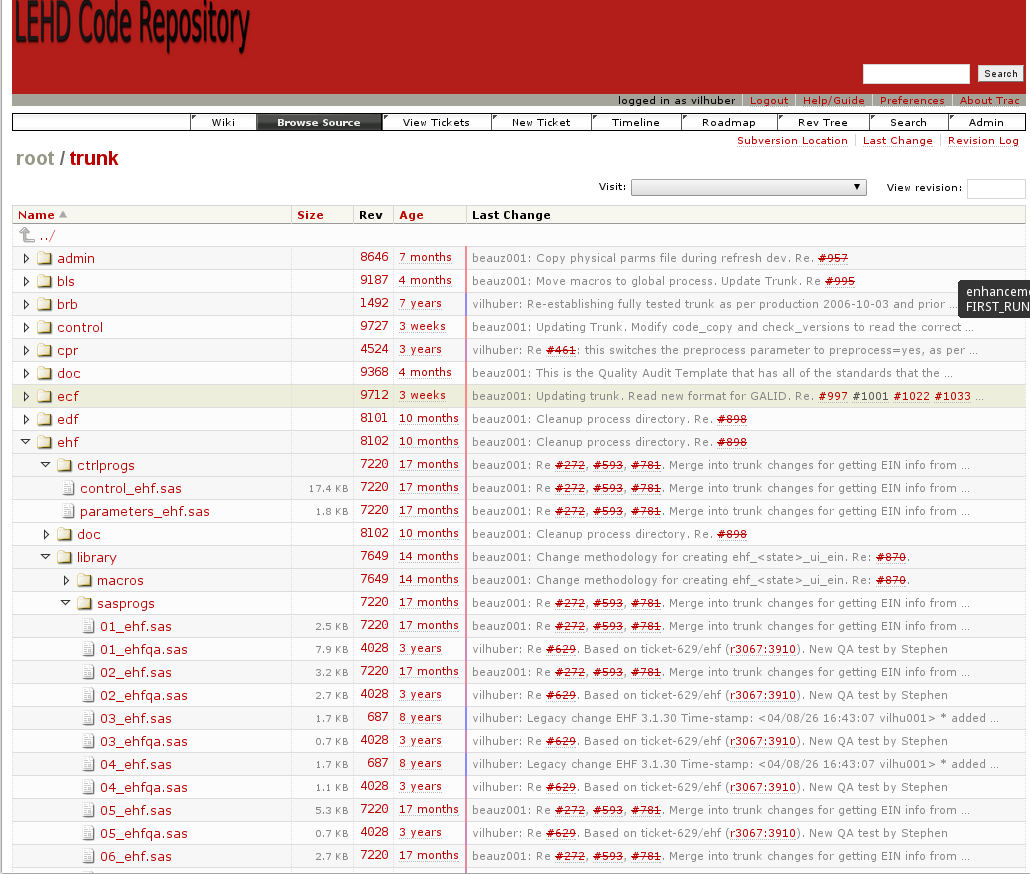
\includegraphics[width=.9\textwidth]{trac-svn-view1.png}
\end{frame}

\begin{frame}{Tracking using web interfaces: SVN}
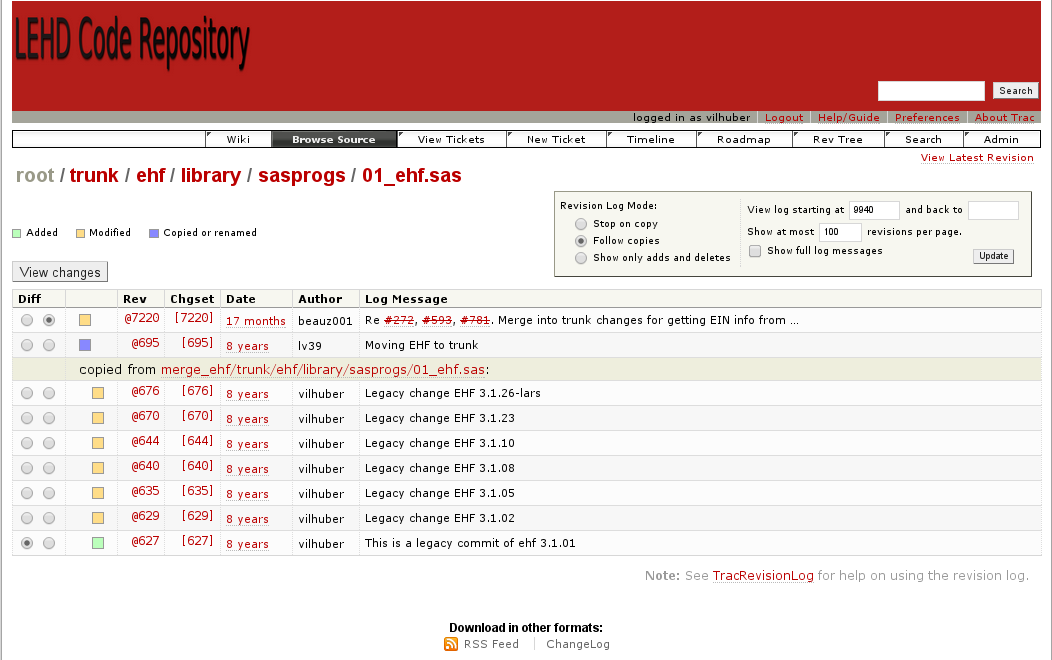
\includegraphics[width=.9\textwidth]{trac-svn-view2.png}
\end{frame}

\begin{frame}{Tracking using web interfaces: SVN}
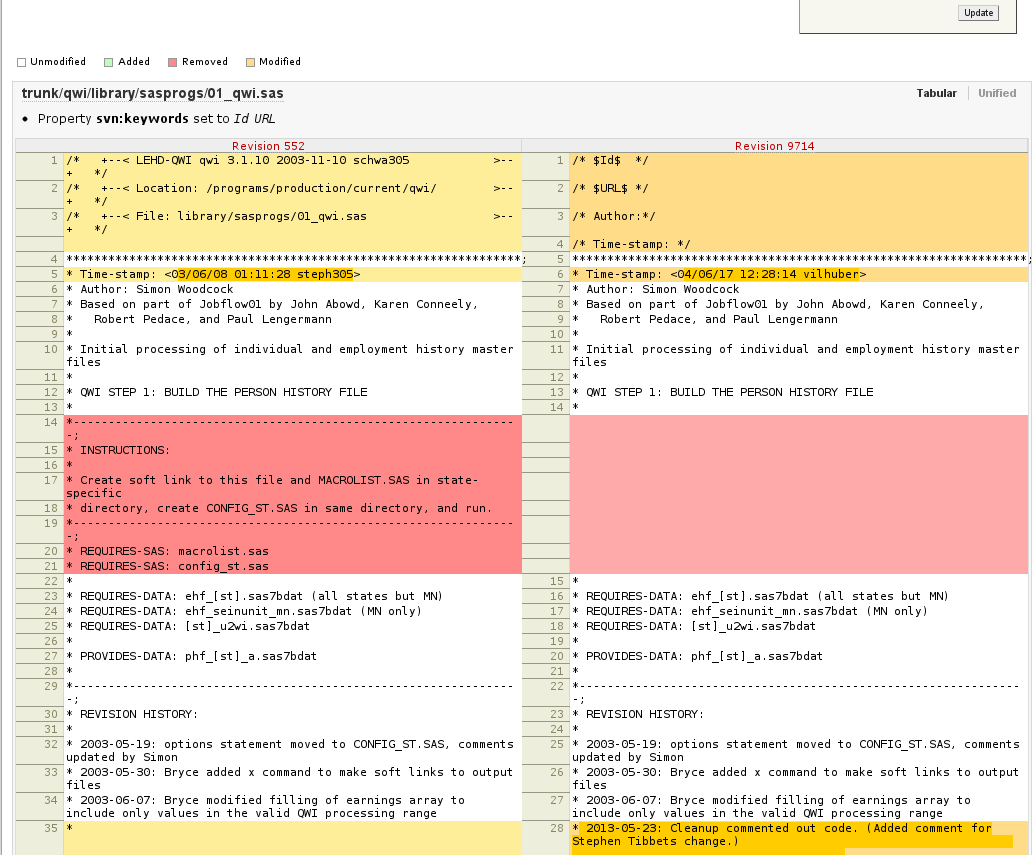
\includegraphics[width=.9\textwidth]{trac-svn-view3.png}
\end{frame}

\begin{frame}{Tracking using web interfaces: SVN}
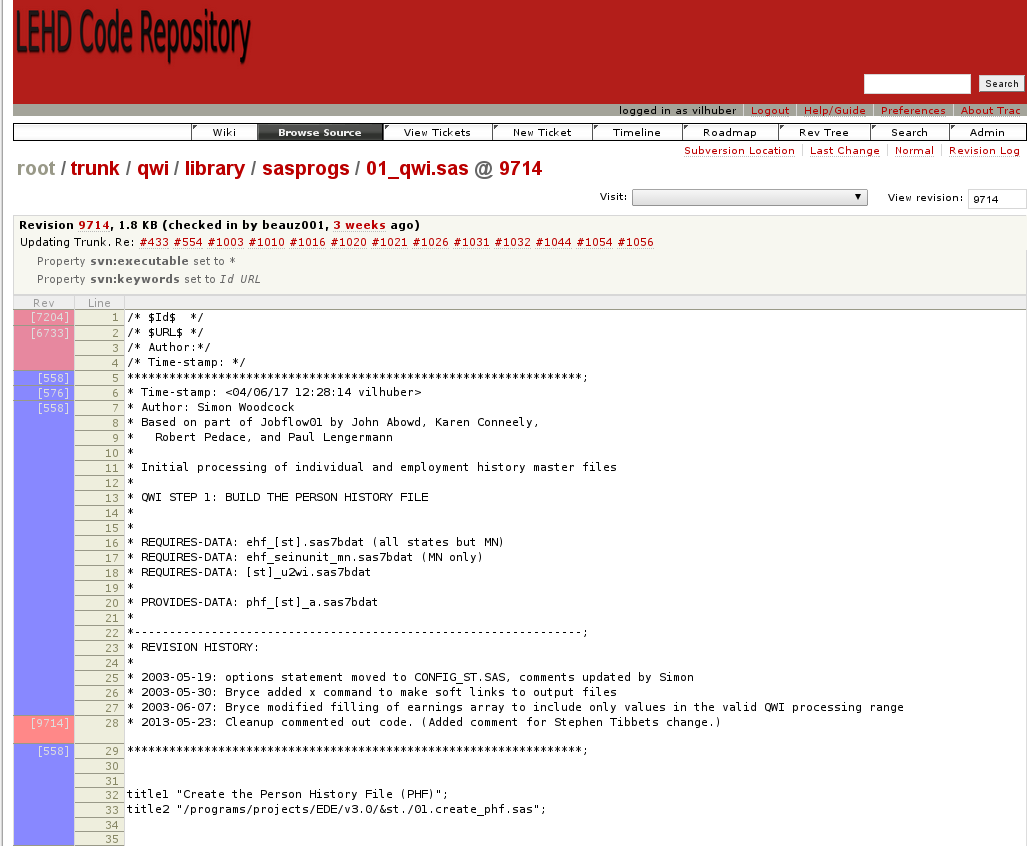
\includegraphics[width=.9\textwidth]{trac-svn-view4.png}
\end{frame}

\begin{frame}{Tracking using web interfaces: git}
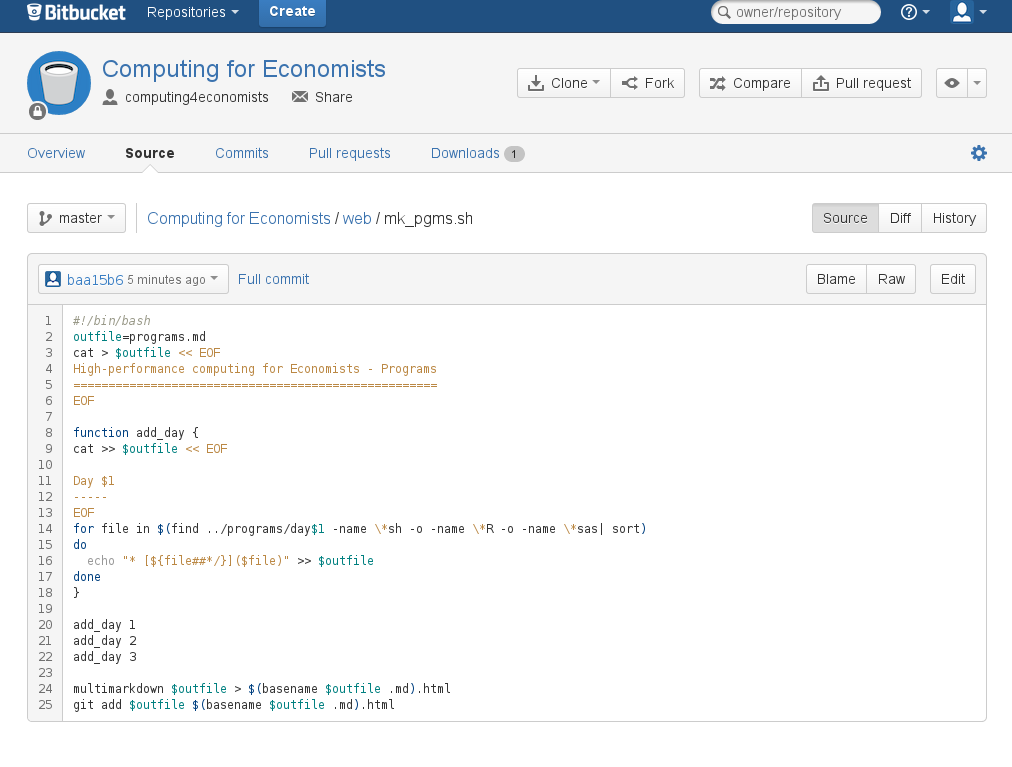
\includegraphics[width=.9\textwidth]{git-view1.png}
\end{frame}

\begin{frame}{Tracking using web interfaces: git}
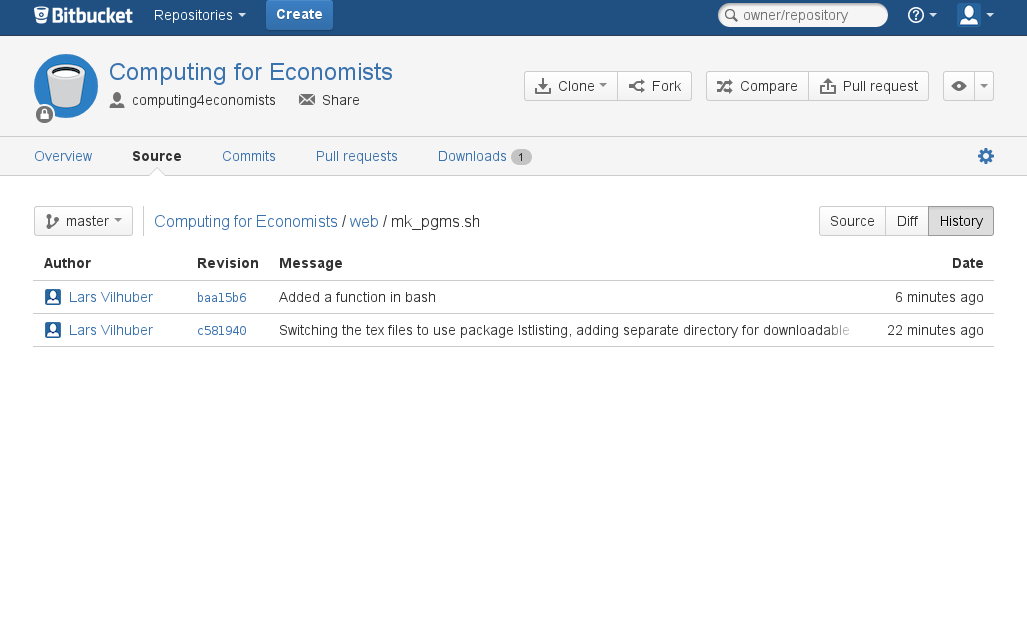
\includegraphics[width=.9\textwidth]{git-view2.png}
\end{frame}

\begin{frame}{Tracking using web interfaces: git}
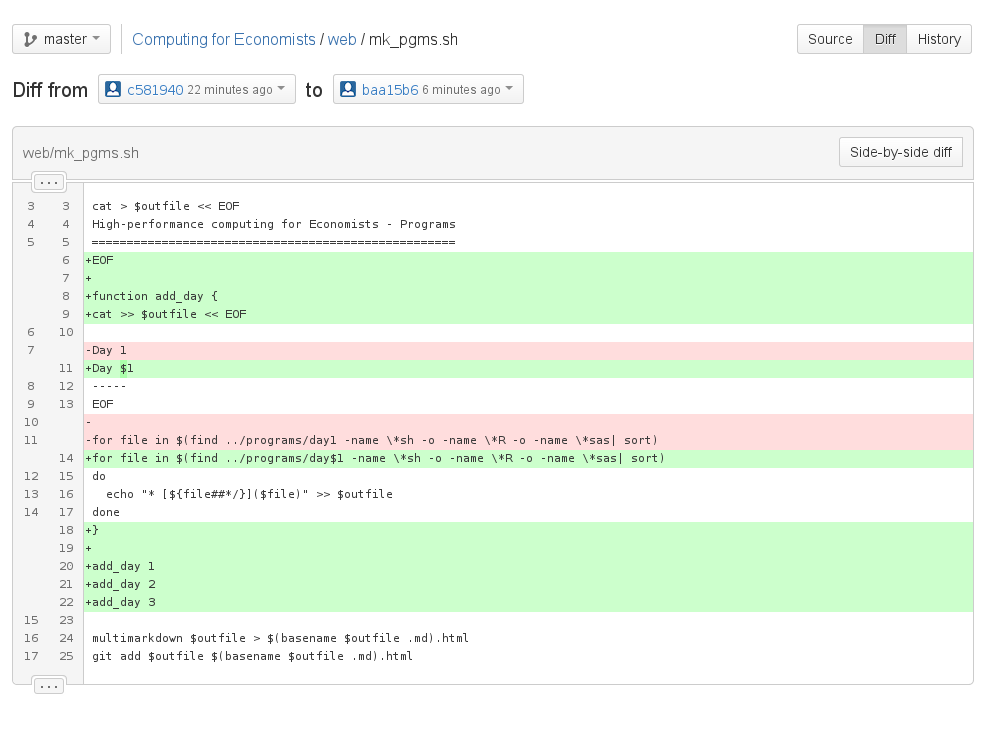
\includegraphics[width=.9\textwidth]{git-view3.png}
\end{frame}


\subsection{Comparing systems}
\begin{frame}[fragile]{Subversion vs. Git}
\small

\begin{block}{Checking out a subdirectory}
\begin{columns}
\begin{column}{.48\textwidth}
\color{red}\rule{\linewidth}{4pt}

SVN
\end{column}%
\hfill%
\begin{column}{.48\textwidth}
\color{blue}\rule{\linewidth}{4pt}

GIT
\end{column}%
\end{columns}
\begin{columns}
\begin{column}{.48\textwidth}
\color{red}
\begin{lstlisting}
svn co ${URL}/sub/directory (name)
\end{lstlisting}
\end{column}%
\hfill%
\begin{column}{.48\textwidth}
\color{blue}\tiny
\begin{lstlisting}
mkdir <repo> && cd <repo>
git init
git remote add -f <name> <url>
git config core.sparsecheckout  true
echo some/dir/ >> .git/info/sparse-checkout
echo another/sub/tree >>  .git/info/sparse-checkout
git pull <remote> <branch>
\end{lstlisting}
{\tiny Source: \href{http://jasonkarns.com/blog/subdirectory-checkouts-with-git-sparse-checkout/}{here}}
\end{column}%

\end{columns}
\end{block}
\end{frame}

\section{Subroutines}
\begin{frame}
\href{day1-3.pdf}{Next section}
\end{frame}

\end{document}